% !TeX root = Stageportfolio.tex



\begin{landscape}
	\subsection{Lessen aan VISO}
	De bijlagen per lesblok (e.g. bordschema, uitgeschreven oplossingen, labo's \ldots) zijn na elk lesblok terug te vinden. 
	\subsubsection{Les 1-2}
	\begin{tabularx}{1.56\textwidth}{|p{0.35\textwidth}|X|}\hline
		\textbf{Administratieve gegevens}\newline\newline
		Kevin Truyaert\newline\newline
		technisch secundair onderwijs\newline
		3e graad, 1ste jaar, Techniek-Wetenschappen\newline
		VVKSO: \href{http://ond.vvkso-ict.com/leerplannen/doc/Toegepaste\%20fysica-2014-041.pdf}{http://ond.vvkso-ict.com/leerplannen /doc/Toegepaste\%20fysica-2014-041.pdf} \newline
		\underline{Lesonderwerp}:\newline `Labo M4: De stroombalans' & \textbf{Doelstellingen}
		\begin{itemize}[itemsep=0.08\baselineskip]
			\item B24: De richting, de zin en de grootte van de Lorentzkracht op een rechte stroomvoerende geleider aangeven en hiermee de magnetische veldsterkte omschrijven. 
			\item AD4 Reflecteren: Over een waarnemingsopdracht/experiment/onderzoek en het resultaat reflecteren.
			\item AD5 Rapporteren: Over een waarnemingsopdracht/experiment/onderzoek en het resultaat rapporteren.
			\item AD10 Meettoestellen en meetnauwkeurigheid: De gepaste toestellen kiezen voor het meten van de behandelde grootheden en de meetresultaten correct aflezen en noteren.
			\item AD 12 Grafieken: Meetresultaten grafisch voorstellen in een diagram en deze interpreteren.
		\end{itemize}
		\underline{Lesdoelen}\newline
		\vspace{-0.75cm}
		\begin{enumerate}[itemsep=0.08\baselineskip]
			\item De leerlingen kunnen de Lorentzkracht toepassen op de specifieke situatie van de stroombalans.
			\item De leerlingen werken samen om een wetenschappelijke opstelling te kunnen bouwen.
			\item De leerlingen voeren de beschreven handelingen uit om tot resultaten te komen.
			\item De leerlingen meten de resultaten nauwkeurig op.
			\item De leerlingen reflecteren over de resultaten.
			\item De leerlingen rapporteren over hun resultaten.
			\item De leerlingen houden bij hun berekeningen rekening met de nauwkeurigheid.
			\item De leerlingen stellen de meetresultaten grafisch voor.
		\end{enumerate} \\\hline
	\end{tabularx}


	\begin{tabularx}{1.56\textwidth}{|p{0.55\textwidth}|X|}
		\hline
		\multirow{2}{0.55\textwidth}{\textbf{Beginsituatie}\newline  
		Er zijn acht leerlingen binnen 5TW. Er heerst een algemene klassfeer. De leerlingen hebben al theorie gekregen  rond en oefeningen gemaakt op de magnetische krachtwerking. \newline\newline Bij dit labo beschikt de school over drie opstellingen van de stroombalans, wat in evenveel groepjes resulteert. De mentor voorziet de verdeling van de groepjes, aangezien dit in een rotatiesysteem verwerkt zit voor andere labo's.\newline\newline Het lokaal is het fysicalokaal waar mogelijkheid is om elektriciteit uit  pilaren te halen die centraal per rij staan. Er zijn voldoende voorzieningen voor het experimentele materiaal. Er is ook een krijtbord en een beamer aanwezig. \newline\newline Dit is mijn eerste les in het tso en is meteen een labo. Als leerkracht ben ik hierdoor wat nerveus (eerste les) maar zeer benieuwd naar het kunnen van de leerlingen, iets wat ik meteen kan testen vanaf mijn eerste les, vanwege het onderwerp. } & \textbf{Acties}\newline  
		
		\\ \cline{2-2}
		  & \textbf{Bronnen}\begin{itemize}
		  	\item Schramme, S. (2018) De stroombalans, labo magnetisme 4
		  	\item Frederiksen (2014), Current Balance 4565.00
		  \end{itemize}\\ \hline
	\end{tabularx}


\newpage
	
%	\begin{tabularx}{1.56\textwidth}{|p{1.5cm}|p{6cm}|X|p{4cm}|}
%		\hline
%		\textbf{Nr. lesdoel } & \textbf{Inhoud (timing)}  & \textbf{Organisatie } & \textbf{Media } \\ \hline
%		&\underline{Herhaling theorie (15 minuten)}\newline
%		De algemene student heeft op dit moment weinig voeling met de te bespreken leerstof, want het is de eerste oefenzitting over dit onderwerp. Dit heb ik zowel de voorbije jaren tijdens mijn oefenzittingen gemerkt als bij de geobserveerde theorielessen. Daarom breng ik de theorie waarop de studenten oefeningen zullen maken nog eens zelf aan bord. Deze behandelt vijf topics: lading, elektrisch veld, elektrische kracht, flux en de elektrische wet van Gauss. Vooral deze laatste vormt een struikelblok voor de studenten. Het is mijn bedoeling om die op verschillende manieren nog eens uitgelegd te hebben.
%		&  \underline{Doceren}\newline 
%		Ik bouw de te gebruiken theorie op door te starten vanuit de eigenschappen van een lading, dat die een elektrisch veld genereren en dat een elektrisch veld op een andere lading inwerkt door middel van de elektrische kracht. Daarna herhaal ik nog kort eens wat elektrische flux is, om dat tot het grootste probleempunt te komen: de elektrische wet van Gauss.\newline
%		Ik wil vooral heel hard benadrukken wat deze wet zegt, door de aparte onderdelen uit te leggen en conceptueel voor te stellen. Ik doe dit vanuit verschillende insteken om zoveel mogelijk studenten mee te hebben. 
%		\newline 
%		Hierna noteer ik de oefeningen op bord die gemaakt kunnen worden. Dit zijn oefeningen 51 t.e.m. 55, 57 en 56, in die volgorde. Ik verwacht dat deze oefeningen door de betere studenten allemaal gemaakt kunnen worden. Ik verwacht dat de meesten zullen vast komen te zitten bij oefening 54 en 55. Deze gaan namelijk over de elektrische wet van Gauss. Oefeningen 57 en 56 kunnen tijdens de volgende les eventueel ook nog aan bod komen. 
%		& Krijtbord (Bordschema, zie bijlage)
%		\\ \hline
%	\end{tabularx}
%
%	
%
%\begin{tabularx}{1.56\textwidth}{|p{1.5cm}|p{6cm}|X|p{4cm}|}
%	\hline
%	\textbf{Nr. lesdoel } & \textbf{Inhoud (timing)}  & \textbf{Organisatie } & \textbf{Media } \\ \hline
%	&\underline{Afsluiten (5 minuten)}\newline 
%	&  \underline{Afsluiten}\newline
%	Ik herhaal nog even kort wat er van de studenten verwacht werd tijdens deze les en wat ze bijgeleerd hebben. Ik zeg ook wat het onderwerp van volgende les is en vraag aan de studenten om de theorie nog even te herhalen.
%	& 
%	\\ \hline
%\end{tabularx}
%	
%	
	
	
\end{landscape}


%\subsection*{Bijlage 1.1: voorbereiding theorie}
%
%\subsection*{Bijlage 1.2: bordschema theorie}
%\begin{center}
%	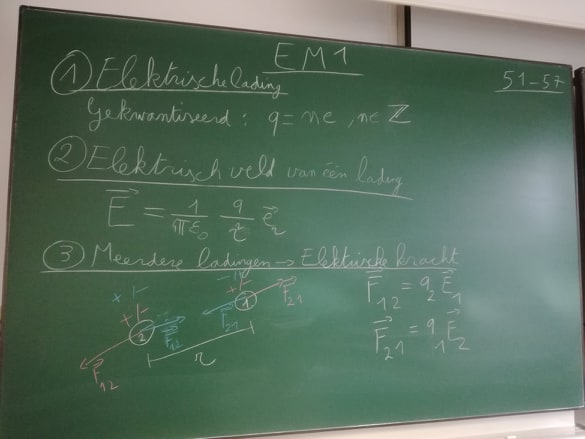
\includegraphics[width=0.9\textwidth]{Bord1a}
%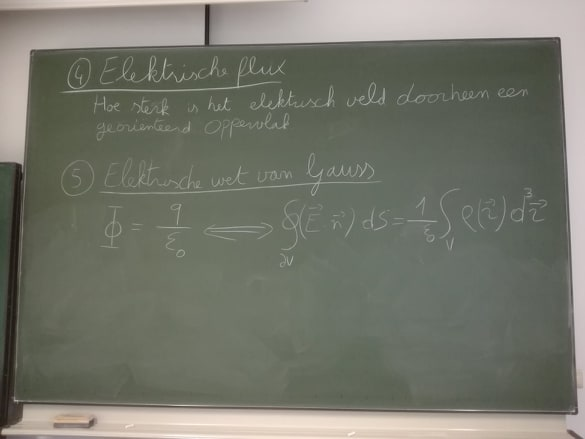
\includegraphics[width=0.9\textwidth]{Bord1b}
%\end{center}
%\newpage
%
%
%\includepdf[scale = 0.8,pages = 17,pagecommand=\subsection*{Bijlage 1.3: opgeloste oefeningen}]{Observaties_OpgelosteOef}
%\includepdf[scale = 0.8,pages =18-20,pagecommand=]{Observaties_OpgelosteOef}
%
%
%
%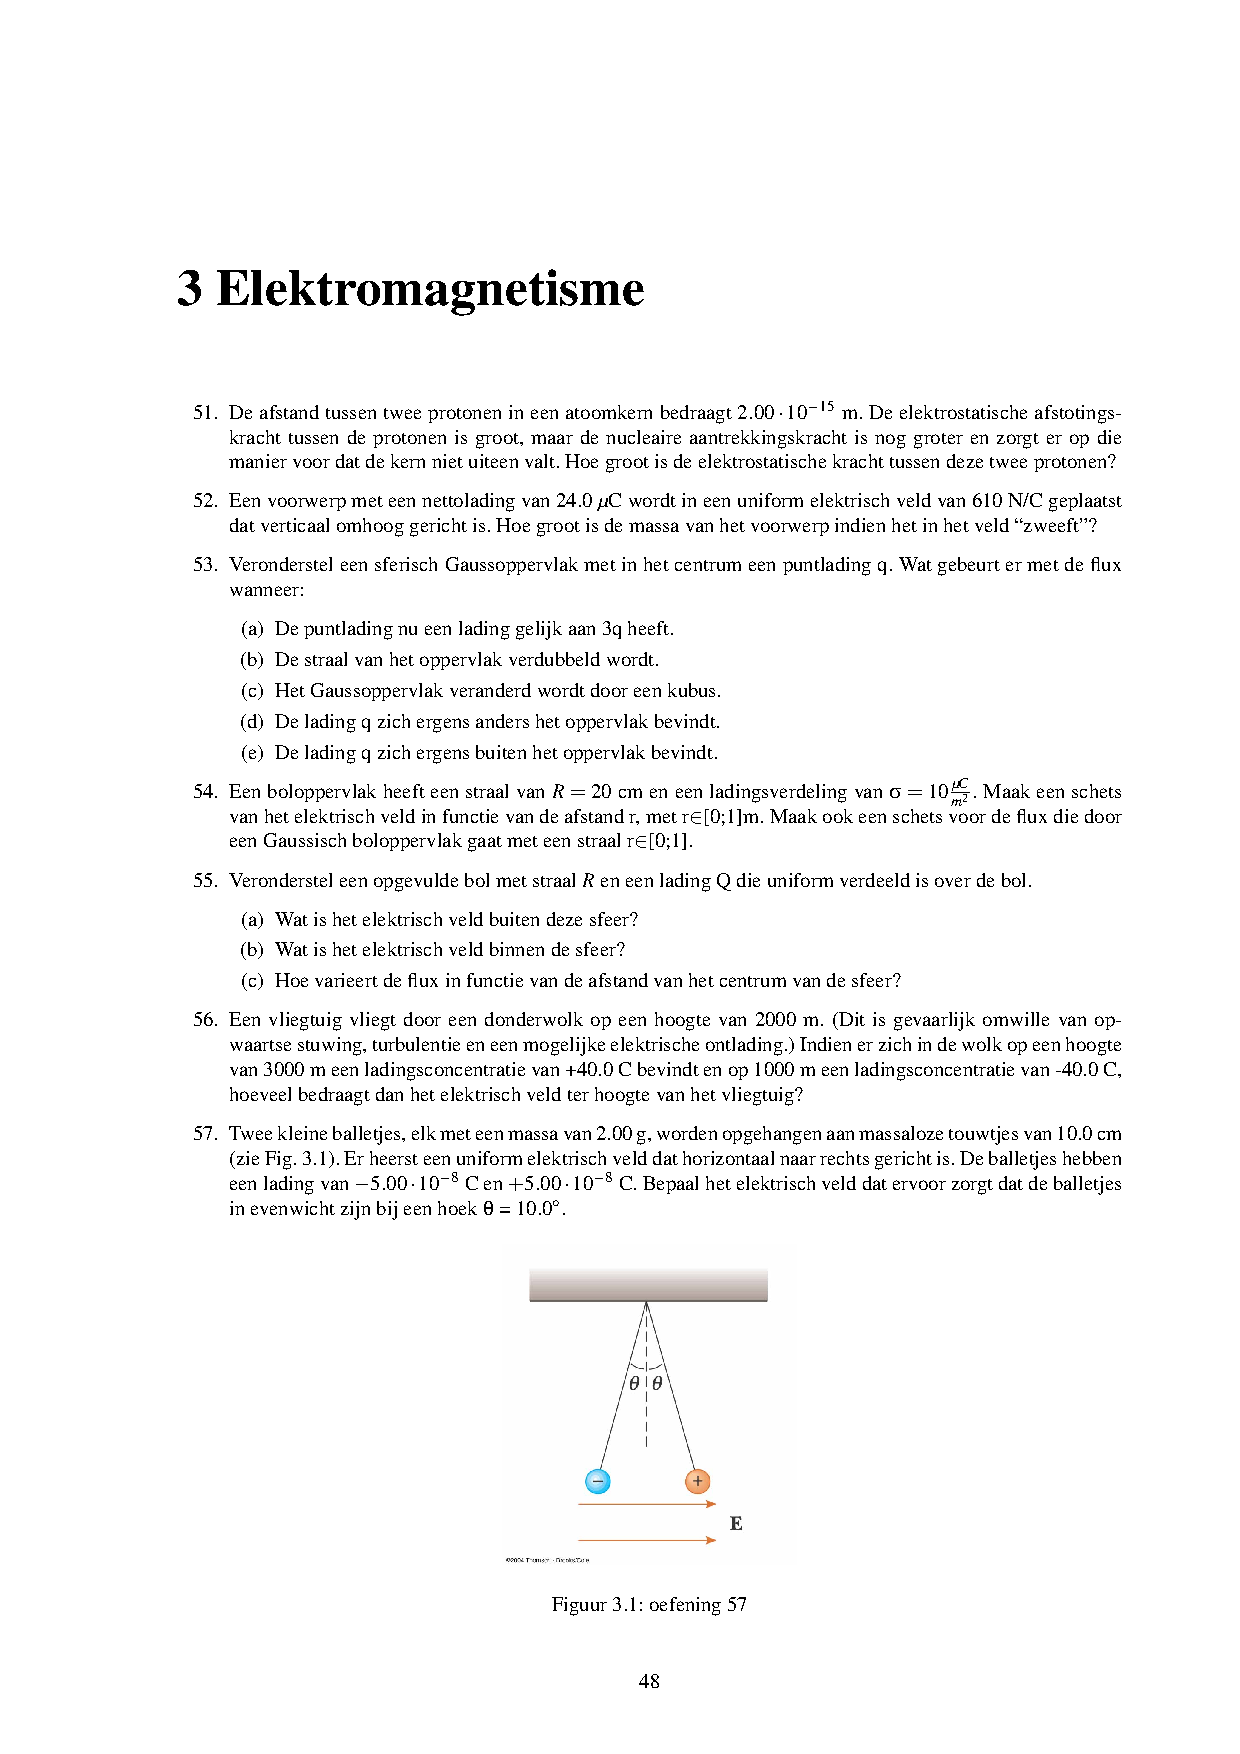
\includepdf[scale = 0.95,pages = 1,pagecommand=\subsection*{Bijlage 1.4: oefeningenbundel elektromagnetisme}]{OefeningenBundel}
%\includepdf[scale = 0.95,pages =2-,pagecommand=]{OefeningenBundel}